\documentclass{article}

\usepackage{tikz} 
\usetikzlibrary{automata, positioning, arrows} 

\usepackage{amsthm}
\usepackage{amsfonts}
\usepackage{amsmath}
\usepackage{amssymb}
\usepackage{fullpage}
\usepackage{color}
\usepackage{parskip}
\usepackage{hyperref}
  \hypersetup{
    colorlinks = true,
    urlcolor = blue,       % color of external links using \href
    linkcolor= blue,       % color of internal links 
    citecolor= blue,       % color of links to bibliography
    filecolor= blue,        % color of file links
    }
    
\usepackage{listings}
\usepackage[utf8]{inputenc}                                                    
\usepackage[T1]{fontenc}      
\usepackage{pdfpages}                                                 

\definecolor{dkgreen}{rgb}{0,0.6,0}
\definecolor{gray}{rgb}{0.5,0.5,0.5}
\definecolor{mauve}{rgb}{0.58,0,0.82}

\lstset{frame=tb,
  language=haskell,
  aboveskip=3mm,
  belowskip=3mm,
  showstringspaces=false,
  columns=flexible,
  basicstyle={\small\ttfamily},
  numbers=none,
  numberstyle=\tiny\color{gray},
  keywordstyle=\color{blue},
  commentstyle=\color{dkgreen},
  stringstyle=\color{mauve},
  breaklines=true,
  breakatwhitespace=true,
  tabsize=3
}

\newtheoremstyle{theorem}
  {\topsep}   % ABOVESPACE
  {\topsep}   % BELOWSPACE
  {\itshape\/}  % BODYFONT
  {0pt}       % INDENT (empty value is the same as 0pt)
  {\bfseries} % HEADFONT
  {.}         % HEADPUNCT
  {5pt plus 1pt minus 1pt} % HEADSPACE
  {}          % CUSTOM-HEAD-SPEC
\theoremstyle{theorem} 
   \newtheorem{theorem}{Theorem}[section]
   \newtheorem{corollary}[theorem]{Corollary}
   \newtheorem{lemma}[theorem]{Lemma}
   \newtheorem{proposition}[theorem]{Proposition}
\theoremstyle{definition}
   \newtheorem{definition}[theorem]{Definition}
   \newtheorem{example}[theorem]{Example}
\theoremstyle{remark}    
  \newtheorem{remark}[theorem]{Remark}

\title{CPSC-406 Report}
\author{Ryan Benner  \\ Chapman University}

\date{\today} 

\begin{document}

\maketitle

\begin{abstract}
\end{abstract}

\setcounter{tocdepth}{3}
\tableofcontents

\section{Introduction}\label{intro}

\section{Week by Week}\label{homework}

\subsection{Week 1}

1. Automata

- machine model which has variety of computations without memory
- traversal (trees, graphs, nodes)
- Turing machine
- traffic light

- parking machine
- mechanical calculators
- streaming
- regular expressions (regex): such as NLP, parsing, coding theory, file management

automata: implement algorithms, admit algorithmic instructions.


2. Computability And complexity

- universal language to analyze algorithms/problems/computations for:
- efficiency/(runtime, spacetime, etc) resource/scaling
- comparison between complexity, hardness of problems
- complexity classes
- big-o-notation
- reducing problems
- P vs NP, sat problems

3. Graph Algorithms

- network theory ( data, mechanical, chemical, operations)

2/6

1. Automata theory

states: positions: (head) $\overrightarrow{l}$  () $\overrightarrow{t}$  (end)

ex.1 parking machine:
charge/hr = 25c
accepted: coins, no change, no 1, 2c coins

states:
- value paid so far (0)
0 -> [5,10,25]

ex.2 valid var names:
1. index 0: letter?
2. index n > 0: letter or digit or symbol

\subsection{Week 2}

\subsubsection*{Notes}

Chapter 2.1 of ITALC discusses the basic model of computation that demonstrates the structure and components of finite automata. It explains that a finite automaton is a simple computational machine which is composed of a set of states, including a start state, and one or more end states. As the automaton reads an input, it transitions between states based on a set of rules, the transition functions. The section uses examples with simple intuition, such as an on/off switch, to show how a system can 'remember' essential information despite its simplicity. Also, it talks about the difference between deterministic and non-deterministic models. A deterministic model is one in which each state has a unique transition for each input, and a non-deterministic model is one where multiple transitions may be possible for one input. Although these two models are very different in practice, they recognize the same set of basic regular language. 

\subsubsection*{Homework}

\underline{Introduction to Automata Theory:}

Homework: Characterize all the accepted words (i.e., describe exactly those words that get recognized).\newline
Answer:  [5, 5, 5, 5, 5], [5, 5, 5, 10], [5, 5, 10, 5], [5, 10, 5, 5], [5, 10, 10], [10, 5, 5, 5], [10, 5, 10], [10, 10, 5]

Homework: Characterize all the accepted words. Can you describe them via a regular expression?\newline
Answer: Any word which ends in 'pay' will result in end state being unlocked

\underline{Deterministic and Non-Deterministic Finite Automata:}

Homework: Determine for the following words, if they are contained in $L_{1}$, $L_{2}$, or $L_{3}$.\newline
Answer:
\begin{table}[h!]
  \centering
  \begin{tabular}{||c c c||} 
   \hline
   word & A\_1 & A\_2 \\ [0.5ex] 
   \hline\hline
   aaa & no  & yes  \\ 
   aab & yes  & no  \\
   aba & no  & no  \\
   abb & no  & no  \\
   baa & no  & yes \\ 
   bab & no & no \\
   bba & no & no \\
   bbb & no & no \\ [1ex] 
   \hline
  \end{tabular}
  \end{table}

Homework: Consider the DFA from above: Consider the paths corresponding to the words $w_{1}$ = 0010, $w_{2}$ = 1101, $w_{3}$ = 1100.\newline
Answer: $w_{1}$ and $w_{2}$ both achieve the end state

\subsubsection*{Comments and Questions}
Because finite automata have limited memory, their ability to recognize more complex language patterns is restricted. Will the range of what is categorized as a finite automaton broaden over time? How could we modify automata to recognize more complex language?


\subsection{Week 3}

\subsubsection*{Notes}

\subsubsection*{Homework}

\underline{Exercise 2, 1-3:}

The file $\mathbf{dfa.py}$ implements a class representing a deterministic finite automaton(DFA) The automaton is defined by a set of states, inputs, transition functions, an initial state, and accepting states, all of which are initialized in the constructor function. The repr method offers a formatted string representation of the DFA for easy inspection. The run method processes an input word by iterating through its characters and transitions between states according to the defined rules. If an undefined transition is encountered or an invalid symbol is detected, the word is rejected. Finally, the refuse method generates a complementary DFA by changing the set of accepting states to accept words that the original DFA rejects.
\newline
The file $\mathbf{dfa-ex01.py}$ implements two DFAs, A1 and A2, and runs each through dfa.py to test them repsectively.

\lstinputlisting[language=Octave]{../labs/py-automata/dfa.py}
\lstinputlisting[language=Octave]{../labs/py-automata/dfa_ex01.py}

\underline{Drawings for Lab Exercise 4, ITALC Exercise 2.2.4}

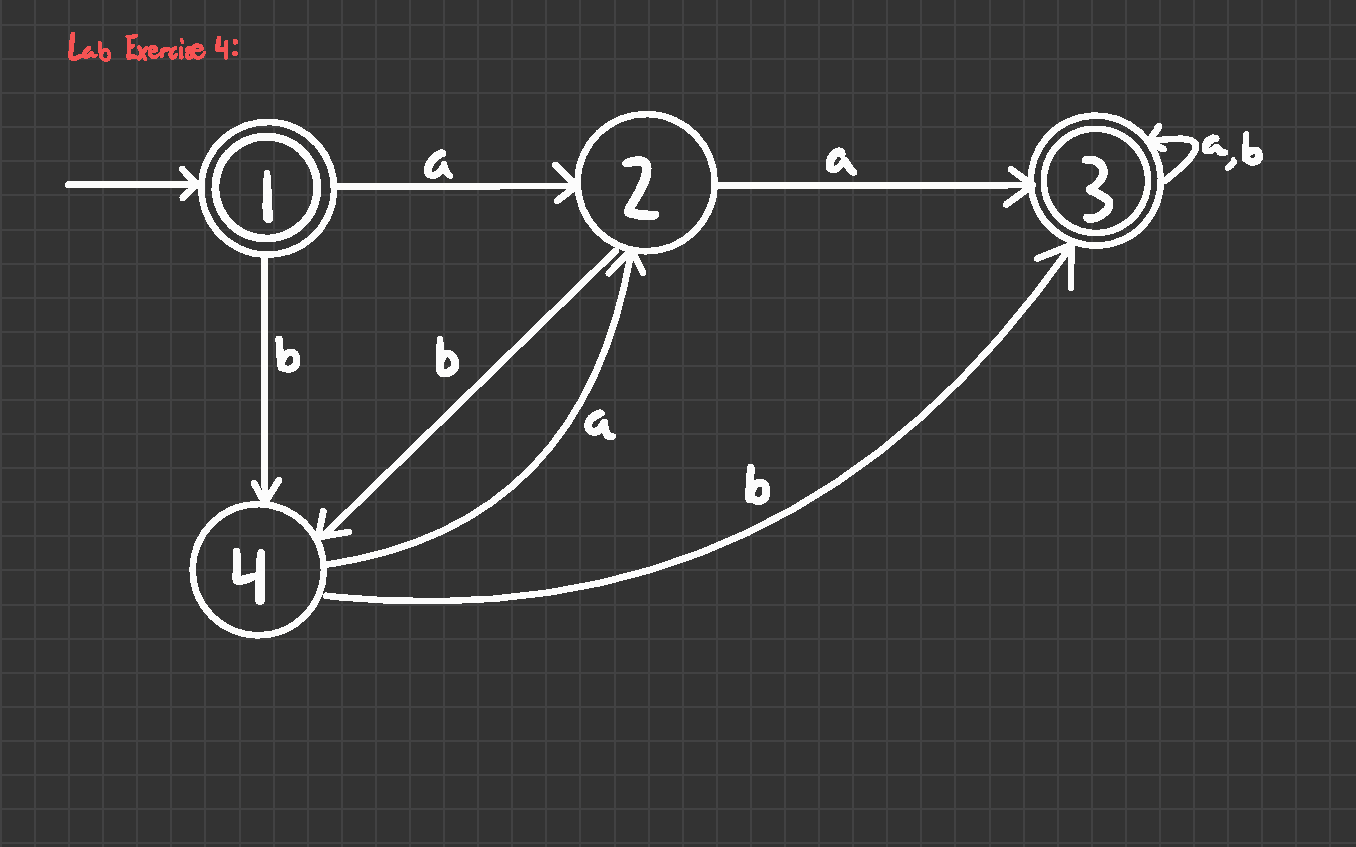
\includepdf[pages=-]{attachments/CPSC406_HW2.pdf}

\subsubsection*{Comments and Questions}

I occasionally find myself struggling to recognize the pattern when first looking at a new DFA. Is there an insightful method or trick to recognizing these patterns more easily?

\subsection{Week 4}

\subsubsection*{Notes}

\subsubsection*{Homework}

\underline{Homework 1}

1. The language of the automata A2 can be described as starting with an a and having an odd length. Any b's that may occur must do so from state 2. This can be described as a regular expression $a((a|b)a)*$.

2. The extended transition functions can be evaluated as follows:

A1:
\begin{itemize}
  \item $\delta_1(1, a) = 2$
  \item $\delta_1(2, b) = 4$
  \item $\delta_1(4, a) = 2$
  \item $\delta_1(2, a) = 3$
\end{itemize}

A2:
\begin{itemize}
  \item $\delta_2(1, a) = 2$
  \item $\delta_2(2, b) = 1$
  \item $\delta_2(1, b) = 3$
  \item $\delta_2(3, a) = 3$
\end{itemize}

\underline{Homework 2}

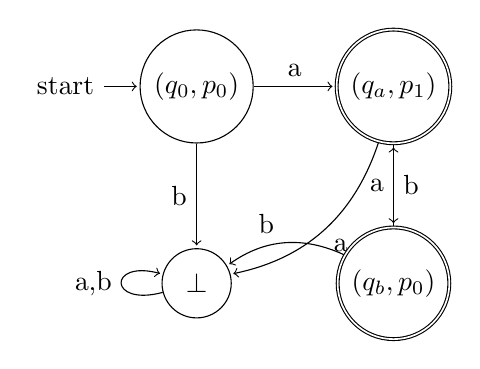
\begin{tikzpicture}[shorten >=1pt,node distance=2.5cm,on grid,auto]
  % Nodes
  \node[state,initial] (q0) {$(q_0,p_0)$};
  \node[state,accepting] (qa) [right=of q0] {$(q_a,p_1)$};
  \node[state,accepting] (qb) [below=of qa] {$(q_b,p_0)$};
  \node[state] (trap) [below=of q0] {$\bot$};
  % Transitions from (q0,p0)
  \path[->]
      (q0) edge node {a} (qa)
           edge node [swap] {b} (trap)
  % Transitions from (q_a,p_1)
      (qa) edge node {b} (qb)
           edge[bend left] node {a} (trap)
  % Transitions from (q_b,p_0)
      (qb) edge node {a} (qa)
           edge[bend right] node [swap] {b} (trap)
  % Trap self-loop
      (trap) edge [loop left] node {a,b} (trap);
\end{tikzpicture}

2. When constructing the product automaton, a word w is processed by both components simultaneously. The word is said to be accepted iff the computation ends in a state $(q,p)$ where q is in F(1) and p is in F(2). This means that w is accepted by both A(1) and A(2), so L(A) can be the intersection between the two. 

3. In the product automaton constrction, the set of states is always $Q_1 * Q_2$ and the transitions are the same. To find an automaton which is the union of the two languages, we change the accepting states. So, a word w is accepted by A' iff it is accepted by at least one of the original automata, which gives L(A') to be the union of L(A1) and L(A2). 

To summarize:

\[
\begin{aligned}
Q &= Q^{(1)}\times Q^{(2)}, \\
\delta((q,p),x) &= (\delta^{(1)}(q,x),\,\delta^{(2)}(p,x)), \\
q_0 &= (q_0^{(1)},q_0^{(2)}), \\
F' &= \Bigl\{(q,p) \in Q^{(1)}\times Q^{(2)} : q\in F^{(1)} \text{ or } p\in F^{(2)}\Bigr\}.
\end{aligned}
\]


\subsubsection*{Comments and Questions}

Do automata with some form of union or intersection have real world applications relating to natural language processing? Could they be used to improve parsing in conversational AI? 

\section{Synthesis}

\section{Evidence of Participation}

\section{Conclusion}\label{conclusion}

\begin{thebibliography}{99}
\bibitem[BLA]{bla} Author, \href{https://en.wikipedia.org/wiki/LaTeX}{Title}, Publisher, Year.
\end{thebibliography}

\end{document}